\documentclass[12pt,aspectratio=169]{beamer}
\usepackage[T1]{fontenc}
\usepackage{lmodern}
\usepackage{amsmath,amssymb,array,booktabs,tabularx,tikz}
% Add language support appropriate to the source, if needed.
% Keep this preamble inline in every delivered deck.
\definecolor{GEInk}{HTML}{132A3E}
\definecolor{GETeal}{HTML}{17675E}
\definecolor{GEFooter}{HTML}{EAF2F1}
\setbeamercolor{background canvas}{bg=white}
\setbeamercolor{normal text}{fg=GEInk,bg=white}
\setbeamercolor{structure}{fg=GETeal}
\setbeamercolor{frametitle}{fg=GEInk}
\setbeamercolor{GE footer}{fg=GETeal,bg=GEFooter}
\setbeamerfont{normal text}{family=\sffamily,size=\normalsize}
\setbeamerfont{title}{size=\huge,series=\bfseries}
\setbeamerfont{subtitle}{size=\normalsize,series=\bfseries}
\setbeamerfont{frametitle}{size=\Large,series=\bfseries}
\setbeamerfont{framesubtitle}{size=\normalsize,series=\mdseries}
\setbeamerfont{GE footer}{size=\footnotesize}
\setbeamersize{text margin left=9mm,text margin right=9mm}
\setbeamertemplate{navigation symbols}{}
\setbeamertemplate{headline}{}
\setbeamercovered{invisible}
\setbeamertemplate{frametitle}{%
  \vskip.5em
  {\usebeamerfont{frametitle}\strut\insertframetitle\strut\par}%
  \ifx\insertframesubtitle\empty\else
    {\usebeamerfont{framesubtitle}\strut\insertframesubtitle\strut\par}%
  \fi
  \vskip.25em
}
\setbeamertemplate{footline}{%
  \begin{beamercolorbox}[wd=\paperwidth,ht=3ex,dp=1.3ex,
    leftskip=9mm,rightskip=9mm]{GE footer}%
    \usebeamerfont{GE footer}\insertsectionhead\hfill
    \insertframenumber/\inserttotalframenumber
  \end{beamercolorbox}%
}
\setlength{\parindent}{0pt}
\setlength{\parskip}{.35em}
\setlength{\tabcolsep}{4pt}
\renewcommand{\arraystretch}{1.22}
\AtBeginEnvironment{frame}{\raggedright}
\addtobeamertemplate{frametitle}{}{%
  \setlength{\abovedisplayskip}{6pt plus 2pt minus 2pt}%
  \setlength{\belowdisplayskip}{6pt plus 2pt minus 2pt}%
  \setlength{\abovedisplayshortskip}{6pt plus 2pt minus 2pt}%
  \setlength{\belowdisplayshortskip}{6pt plus 2pt minus 2pt}%
}

\usepackage{pgfplots}
\pgfplotsset{compat=1.18}
\newif\ifGTenHighlights
\GTenHighlightstrue
% \GTenHighlightsfalse % Uncomment to disable instructional highlights.
\tikzset{ge marker/.style={rectangle,rounded corners=1mm,draw=none,
  fill=#1,fill opacity=.32,text opacity=1,text=GEInk,
  inner xsep=.6mm,inner ysep=.3mm,outer sep=0pt}}
\makeatletter
\newcommand{\GEHighlightMath}[2]{%
  \tikz[baseline=(gehl.base)]\node[ge marker=\GECurrentRole]
    (gehl) {$\m@th#1#2$};}
\newcommand{\GEHighlight}[2]{%
  \ifGTenHighlights\begingroup\def\GECurrentRole{#1}%
  \ifmmode\mathpalette\GEHighlightMath{#2}%
  \else\tikz[baseline=(gehl.base)]\node[ge marker=#1](gehl){#2};\fi
  \endgroup\else#2\fi}
\makeatother
% Keep rows, rules, and table structure outside this space-reserving command.
\newcommand{\GERevealCell}[2]{\leavevmode\visible<#1->{#2}}


\definecolor{Mass}{HTML}{86BFF0}
\definecolor{Cumulative}{HTML}{43A5C9}
\definecolor{Translation}{HTML}{86BFF0}
\definecolor{Quantity}{HTML}{FFBB55}
\definecolor{Outcome}{HTML}{BC9DE0}
\colorlet{cTwoMassColor}{blue!75!black}
\colorlet{cTwoCDFColor}{cyan!65!blue!80!black}
\colorlet{cTwoGuideColor}{cTwoMassColor!35}
\ifGTenHighlights\else
  \colorlet{cTwoMassColor}{black}
  \colorlet{cTwoCDFColor}{black}
  \colorlet{cTwoGuideColor}{gray}
\fi
\newcommand{\GELegendCell}[2]{\GERevealCell{#1}{#2}}
\newcommand{\GEFullLegendCell}[2]{\GERevealCell{1}{#2}}
\newcommand{\GEGeneralNotationLegend}{\begingroup\small
\begin{tabularx}{\linewidth}{@{}>{\raggedright\arraybackslash}p{.18\linewidth}>{\raggedright\arraybackslash}p{.16\linewidth}>{\raggedright\arraybackslash}p{.26\linewidth}>{\raggedright\arraybackslash}X@{}}
\toprule Symbol or notation & Concept & Definition & Meaning in the introductory examples\\\midrule
\GELegendCell{1}{\GEHighlight{Quantity}{$X,x,a$}} & \GELegendCell{1}{\GEHighlight{Quantity}{Quantity}} & \GELegendCell{1}{Variable; value or cutoff.} & \GELegendCell{1}{Payment: fee in \GEHighlight{Quantity}{USD}.}\\
\GELegendCell{1}{\GEHighlight{Quantity}{$S_X$}} & \GELegendCell{1}{\GEHighlight{Quantity}{Support}} & \GELegendCell{1}{Distinct values with positive mass.} & \GELegendCell{1}{Payment: \GEHighlight{Quantity}{$\{0,1\}$}.}\\
\GELegendCell{1}{\GEHighlight{Mass}{$p_X(x)$}} & \GELegendCell{1}{\GEHighlight{Mass}{PMF}} & \GELegendCell{1}{$P(X=x)$; one value; unitless.} & \GELegendCell{1}{Payment: \GEHighlight{Mass}{$p_X(1)$}$=$\GEHighlight{Mass}{$0.75$}; blue stems.}\\
\GELegendCell{1}{\GEHighlight{Cumulative}{$F_X(x)$}} & \GELegendCell{1}{\GEHighlight{Cumulative}{CDF}} & \GELegendCell{1}{$P(X\leq x)$; through cutoff; unitless.} & \GELegendCell{1}{Payment: \GEHighlight{Cumulative}{$F_X(1)$}$=$\GEHighlight{Cumulative}{$1$}; related blue steps.}\\
\bottomrule\end{tabularx}\endgroup}
\newcommand{\GEGraphNotationLegend}{\begingroup\small
\begin{tabularx}{\linewidth}{@{}>{\raggedright\arraybackslash}p{.18\linewidth}>{\raggedright\arraybackslash}p{.16\linewidth}>{\raggedright\arraybackslash}p{.26\linewidth}>{\raggedright\arraybackslash}X@{}}
\toprule Symbol or notation & Concept & Definition & Meaning in the introductory examples\\\midrule
\GELegendCell{1}{\GEHighlight{Cumulative}{$F_X(a^-)$}} & \GELegendCell{1}{Height before $a$} & \GELegendCell{1}{Mass strictly below $a$; unitless.} & \GELegendCell{1}{Payment: before 1 USD, height \GEHighlight{Cumulative}{0.25}.}\\
\GELegendCell{1}{\GEHighlight{Mass}{$p_X(a)$}} & \GELegendCell{1}{Translated mass} & \GELegendCell{1}{From $F_X(a^-)$; pale dashed stem.} & \GELegendCell{1}{Payment: same mass and length.}\\
\GELegendCell{1}{Filled / open dots} & \GELegendCell{1}{CDF endpoints} & \GELegendCell{1}{Filled: included; open: excluded.} & \GELegendCell{1}{Payment: upper / lower heights.}\\\bottomrule
\end{tabularx}\endgroup}
\pgfplotsset{cTwoCDF/.style={width=.94\linewidth,height=4cm,
scale only axis=false,axis lines=left,ymin=-.055,ymax=1.1,
ytick={0,.25,.5,.75,1},grid=major,grid style={gray!15},
tick label style={font=\small},label style={font=\small},
ylabel={\GEHighlight{Cumulative}{$F_X(x)$}},clip=false}}

% Local supplementary representations; shared bar graph macros are unchanged.
\pgfplotsset{cTwoCombined/.style={width=.98\linewidth,height=4.5cm,
every axis plot/.append style={forget plot},axis lines=left,x axis line style={->},ymin=-.035,ymax=1.13,
ytick={0,.25,.5,.75,1},ylabel={Probability},grid=major,
grid style={gray!15},tick label style={font=\small},
label style={font=\small},clip=false,
legend style={at={(.5,-.2)},anchor=north,legend columns=3,
font=\footnotesize,draw=none,cells={anchor=west}},
},cTwoMass/.style={cTwoMassColor,thick},
cTwoPhantom/.style={cTwoGuideColor,densely dashed,line width=1.5pt},
cTwoStep/.style={cTwoCDFColor,thick},
cTwoIncluded/.style={only marks,mark=*,cTwoCDFColor,mark size=1.1pt},
cTwoExcluded/.style={only marks,mark=*,cTwoCDFColor,
mark options={fill=white},mark size=1.1pt}}
% Arguments: supported value, exact mass, cumulative height immediately before it.
% Only a vertical translation is applied: upper height = lower height + mass.
\newcommand{\cTwoPhantom}[3]{%
\addplot[cTwoPhantom] coordinates {(#1,#3)(#1,{#3+#2})};
\addplot[only marks,mark=*,cTwoGuideColor,mark size=1.8pt]
coordinates {(#1,{#3+#2})};}
\newcommand{\cTwoMass}[2]{%
\addplot[cTwoMass] coordinates {(#1,0)(#1,#2)};
\addplot[only marks,mark=*,cTwoMassColor,mark size=1.5pt]
coordinates {(#1,#2)};}
\newcommand{\cTwoConnectionReading}{%
\textbf{How to read the overlay.} Blue PMF stems show isolated masses at the
listed values; their vertical segments do not assign positive probability
to every point along a segment. Each pale dashed stem is the same mass
translated vertically from $0$ to $F_X(a^-)$, without moving its horizontal
coordinate or changing its length. Its top is $F_X(a)$, so
$F_X(a)-F_X(a^-)=p_X(a)$. These guides are neither extra masses nor extra
CDF values at the cutoff. Blue CDF filled points give the CDF values; blue CDF open
points exclude the lower heights. At the smallest support value the
translation is zero: the pale copy lies behind the blue PMF stem. Pale top
dots lie behind the blue endpoint markers, which take visual priority.}


\title{Constructing PMF and CDF Tables and Graphs}
\subtitle{Grade 10 · Term 2 · Lesson 1 · 2026--2027}
\author{}\date{}
\newcommand{\GEOfficialCriterion}{\textbf{C2:} Interprets PMFs and CDFs by verifying their defining properties and using them to calculate point, interval, cumulative, and complementary probabilities in financial contexts.}
\setbeamertemplate{title page}{\raggedright\vfill{\color{GETeal}\usebeamerfont{subtitle}\insertsubtitle\par}\medskip{\color{GEInk}\usebeamerfont{title}\inserttitle\par}\bigskip{\normalsize\GEOfficialCriterion\par}\vfill}
% SOURCE MAP: source G10_T2_L1_C2_practice_activity.tex.
% Complete introduction: sec:intro through immediately before sec:reference.
% Selected sole additional example: prob:fees through before prob:bike;
% solutions sol:fees-1 and sol:fees-2; shared cTwoConnectionReading decoded inline.
% Frames: metadata; two opening notation-reference frames; sec:intro;
% prob:fees (statement, two tasks, full solutions, connection);
% summary from the same source allowance; concise closing legend.
% No explicit key terms/highlight guide or quick checks occur in introduction.
% Palette follows C1 quantities and C2 related probability roles.
\begin{document}
\section{Introduction}
\begin{frame}\titlepage\end{frame}
\begin{frame}[t]{General notation table legend}\GEGeneralNotationLegend\end{frame}
\begin{frame}[t]{Notation reference: graph conventions}\GEGraphNotationLegend\end{frame}
\begin{frame}[t]{One payment: what fee is recorded?}
A shop receives one payment: cash with probability 0.25, debit card with probability 0.45, or credit card with probability 0.30. These are the only methods.

Cash has no processing fee; either card costs the shop 1 USD.

\medskip What numerical results can the shop record?

\visible<2->{The fee is either zero or one dollar. A PMF separates numerical results; a CDF accumulates their probabilities from left to right.}

\visible<3->{All data are hypothetical. Amounts are in USD; probabilities have no units. Keep exact fractions or terminating decimals.}
\end{frame}
\begin{frame}[t]{Payment fee: the two tasks}
\textbf{Task 1 --- PMF table and graph.} Write the probability mass function (PMF) as a table and represent it graphically. Define the random variable, its units and support within this task.

\medskip\textbf{Task 2 --- CDF table and graph.} Write the cumulative distribution function (CDF) as a table and represent it graphically.
\end{frame}
\begin{frame}[t]{Payment fee: group equal numerical values}
How do cash, debit and credit map to fees?
\visible<2->{\GEHighlight{Quantity}{$X$} is the \GEHighlight{Quantity}{processing fee} for one payment, in \GEHighlight{Quantity}{USD}. Cash maps to \GEHighlight{Quantity}{0}; debit and credit both map to \GEHighlight{Quantity}{1}.}
\[\begin{aligned}
\visible<3->{p_X(0)&=\GEHighlight{Mass}{0.25},}\\
\visible<4->{p_X(1)&=\GEHighlight{Mass}{0.45}+\GEHighlight{Mass}{0.30}=\GEHighlight{Mass}{0.75}.}
\end{aligned}\]
\visible<4->{The card events are mutually exclusive, so their probabilities add.}

\visible<5->{$S_X=\{0,1\}$; $p_X(x)=0$ elsewhere.}
\end{frame}
\begin{frame}[t]{Payment fee: PMF table and graph}
\begin{columns}[T,onlytextwidth]\begin{column}{.36\textwidth}\begin{tabular}{cc}\toprule \GEHighlight{Quantity}{$x$ (USD)}&\GEHighlight{Mass}{$p_X(x)$}\\\midrule\GEHighlight{Quantity}{0}&\GEHighlight{Mass}{0.25}\\\GEHighlight{Quantity}{1}&\GEHighlight{Mass}{0.75}\\\bottomrule\end{tabular}\end{column}\begin{column}{.60\textwidth}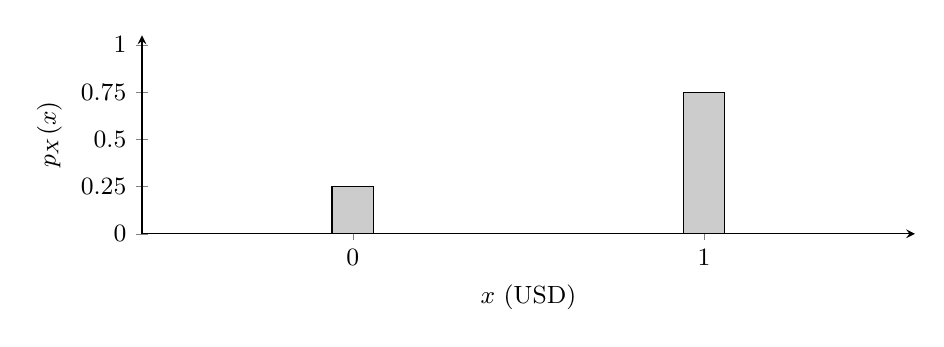
\begin{tikzpicture}\begin{axis}[width=.94\linewidth,height=4.1cm,axis lines=left,ymin=0,ymax=1.05,ytick={0,.25,.5,.75,1},xmin=-.6,xmax=1.6,xtick={0,1},xlabel={\GEHighlight{Quantity}{$x$ (USD)}},ylabel={\GEHighlight{Mass}{$p_X(x)$}},tick label style={font=\small},label style={font=\small}]\addplot[ybar,bar width=15pt,draw=cTwoMassColor,fill=cTwoMassColor!20] coordinates {(0,0.25) (1,0.75)};\end{axis}\end{tikzpicture}\end{column}\end{columns}All masses are positive; $0.25+0.75=1$. Each mass keeps its numerical position and original spacing.
\end{frame}
\begin{frame}[t]{Payment fee: accumulate through the cutoff}
What does $F_X(x)=P(X\leq x)$ include?

\visible<2->{Add masses at values no greater than the cutoff, in increasing support order. Below the minimum, no mass is included.}
\[\begin{aligned}\visible<3->{F_X(0)&=\GEHighlight{Cumulative}{0.25},}\\\visible<4->{F_X(1)&=\GEHighlight{Cumulative}{0.25}+\GEHighlight{Mass}{0.75}=\GEHighlight{Cumulative}{1}.}\end{aligned}\]
\end{frame}
\begin{frame}[t]{Payment fee: CDF table and step graph}
\begin{columns}[T,onlytextwidth]\begin{column}{.36\textwidth}\begin{tabular}{cc}\toprule Cutoff interval & \GEHighlight{Cumulative}{$F_X(x)$} \\\midrule
$x<0$ & $\GEHighlight{Cumulative}{0}$ \\
$0\leq x<1$ & $\GEHighlight{Cumulative}{0.25}$ \\
$x\geq 1$ & $\GEHighlight{Cumulative}{1}$ \\
\bottomrule\end{tabular}\end{column}\begin{column}{.60\textwidth}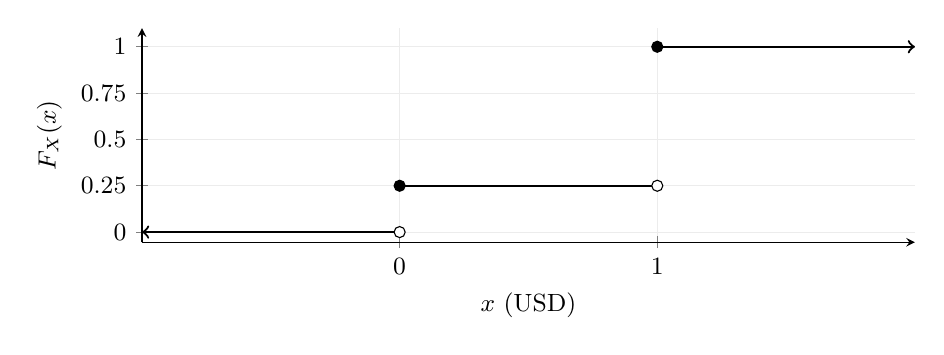
\begin{tikzpicture}\begin{axis}[cTwoCDF,width=.94\linewidth,height=4.3cm,xmin=-1,xmax=2,xtick={0,1},xlabel={\GEHighlight{Quantity}{$x$ (USD)}}]
\addplot[cTwoCDFColor,thick,<-] coordinates {(-1,0)(0,0)};
\addplot[cTwoCDFColor,thick] coordinates {(0,0.25)(1,0.25)};
\addplot[cTwoCDFColor,thick,->] coordinates {(1,1)(2,1)};
\addplot[only marks,mark=*,cTwoCDFColor,mark size=2pt] coordinates {(0,0.25)(1,1)};
\addplot[only marks,mark=*,cTwoCDFColor,mark options={fill=white},mark size=2pt] coordinates {(0,0)(1,0.25)};
\end{axis}\end{tikzpicture}\end{column}\end{columns}
\end{frame}
\begin{frame}[t]{Payment fee: verify the CDF}
Why is this a valid cumulative distribution?

\visible<2->{Nonnegative jumps make it nondecreasing. Filled left/open right endpoints give right-continuity.}

\visible<3->{Tails at 0 and 1 give limits 0 and 1; 1 is attained at the maximum.}

\visible<4->{Jumps $0.25,\ 0.75$ match the PMF. The accumulated height at 0 includes cash payments only.}
\end{frame}
\begin{frame}[t]{From bars to stems}
\begin{columns}[T,onlytextwidth]\begin{column}{.485\textwidth}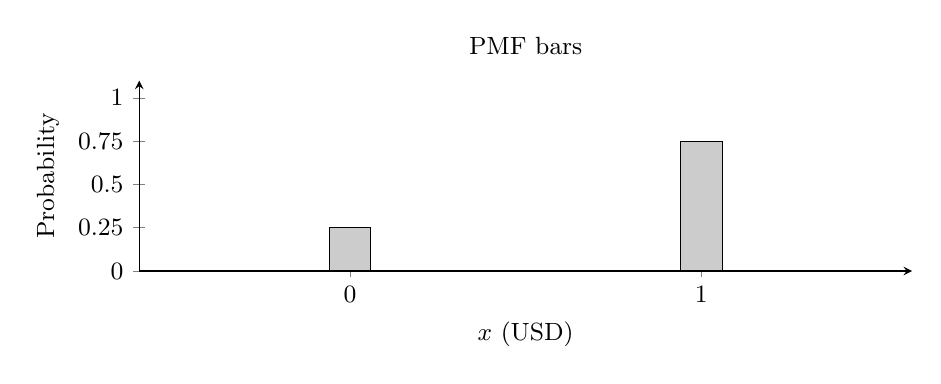
\begin{tikzpicture}\begin{axis}[width=.94\linewidth,height=4cm,
xmin=-.6,xmax=1.6,ymin=0,ymax=1.1,xtick={0,1},ytick={0,.25,.5,.75,1},
axis lines=left,xlabel={\GEHighlight{Quantity}{$x$ (USD)}},ylabel={Probability},title={\small PMF bars},
tick label style={font=\small},label style={font=\small}]
\addplot[ybar,bar width=15pt,draw=cTwoMassColor,fill=cTwoMassColor!20]
coordinates {(0,.25)(1,.75)};
\end{axis}\end{tikzpicture}\end{column}\begin{column}{.485\textwidth}\begin{tikzpicture}\begin{axis}[width=.94\linewidth,height=4cm,
xmin=-.6,xmax=1.6,ymin=0,ymax=1.1,xtick={0,1},ytick={0,.25,.5,.75,1},
axis lines=left,xlabel={\GEHighlight{Quantity}{$x$ (USD)}},ylabel={Probability},title={\small PMF stems},
tick label style={font=\small},label style={font=\small}]
\cTwoMass{0}{.25}\cTwoMass{1}{.75}
\end{axis}\end{tikzpicture}\end{column}\end{columns}Keep each supported value at the same horizontal coordinate. A stem runs from $0$ to $p_X(x)$, with a filled top dot. Height gives mass at one value; bar width and area play no role. The distribution and both scales stay the same.
\end{frame}
\begin{frame}[t]{A CDF jump is a probability mass}
What changes when the cutoff reaches $a$?

\visible<2->{$F_X(a^-)$ is the cumulative probability immediately before $a$: it includes supported values strictly smaller than $a$, but not $a$ itself.}
\[\visible<3->{F_X(a)-F_X(a^-)=\GEHighlight{Mass}{p_X(a)}.}\]
\visible<4->{Before 1 USD the height is $0.25$; at 1 USD it becomes $1$.}
\[\visible<5->{1-0.25=0.75=p_X(1).}\]
\end{frame}
\begin{frame}[t]{Payment fee: the same distribution}
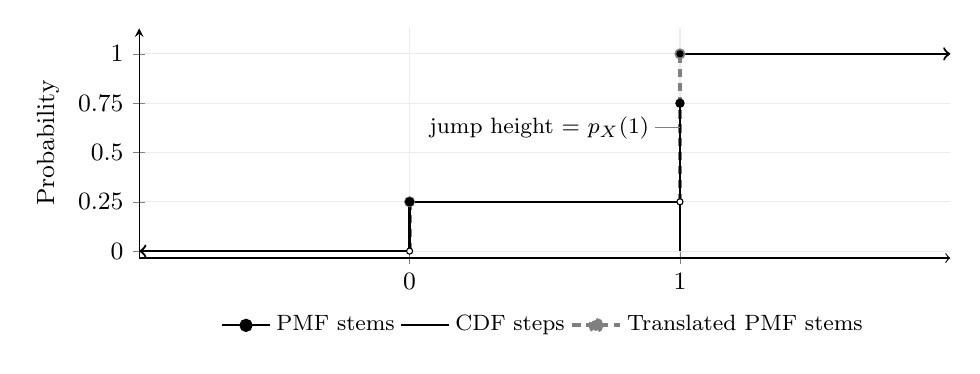
\begin{tikzpicture}
\begin{axis}[cTwoCombined,xmin=-1,xmax=2,xtick={0,1},xlabel={\GEHighlight{Quantity}{$x$ (USD)}}]
\cTwoPhantom{0}{.25}{0}
\cTwoPhantom{1}{.75}{1/4}
\cTwoMass{0}{.25}
\cTwoMass{1}{.75}
\addplot[cTwoStep,<-] coordinates {(-1,0)(0,0)};
\addplot[cTwoStep] coordinates {(0,1/4)(1,1/4)};
\addplot[cTwoStep,->] coordinates {(1,1)(2,1)};
\addplot[cTwoExcluded] coordinates {(0,0)(1,1/4)};
\addplot[cTwoIncluded] coordinates {(0,1/4)(1,1)};
\node[anchor=east,xshift=-9pt,font=\footnotesize,fill=white,inner sep=2pt] (jumpLabel) at (axis cs:1,5/8) {jump height = $p_X(1)$};
\draw[gray,thin] (jumpLabel.east) -- (axis cs:1,5/8);
\addlegendimage{cTwoMass,mark=*}\addlegendentry{PMF stems}
\addlegendimage{cTwoStep}\addlegendentry{CDF steps}
\addlegendimage{cTwoPhantom,mark=*}\addlegendentry{Translated PMF stems}
\end{axis}\end{tikzpicture}\par\medskip At $a=1$ USD, the 1 USD fee adds the probability of both card methods: $1-0.25=0.75=p_X(1)$.
\end{frame}
\begin{frame}[t]{How to read the connection}
Blue PMF stems show isolated masses at the listed values; their vertical segments assign no probability to other points on the segment.

Each pale dashed stem is the same mass translated from $0$ to $F_X(a^-)$, keeping its horizontal coordinate and length. Its top is $F_X(a)$.

The guides are neither extra masses nor extra CDF values. Blue CDF filled points give CDF values; blue CDF open points exclude the lower heights.
\end{frame}
\begin{frame}[t]{Reading overlapping markers}
At the smallest supported value, the translation is zero: the pale copy lies behind the blue PMF stem.

Pale top dots lie behind blue endpoint markers, which take visual priority.

\medskip The connection is always
\[F_X(a)-F_X(a^-)=p_X(a).\]
\end{frame}
\section{School shop}
\begin{frame}[t]{Worked example: school shop processing fees}
A school shop receives one payment. Exactly four methods are possible: cash (10\%), debit card (20\%), credit card (30\%), or mobile wallet (40\%).

The shop pays no processing fee for cash, 1 USD for either type of card, and 2 USD for a mobile wallet. These are the only processing charges.

Record the processing fee for this payment.
\end{frame}
\begin{frame}[t]{School shop: the two tasks}
\textbf{Task 1 --- PMF table and graph.} Write the probability mass function (PMF) as a table and represent it graphically. Define the random variable, its units and support within this task.

\medskip\textbf{Task 2 --- CDF table and graph.} Write the cumulative distribution function (CDF) as a table and represent it graphically.
\end{frame}
\begin{frame}[t]{School shop: define and group}
How do the four payment methods become numerical values?

\visible<2->{\GEHighlight{Quantity}{$X$} is the \GEHighlight{Quantity}{processing fee} for one school-shop payment, in \GEHighlight{Quantity}{USD}. Cash maps to \GEHighlight{Quantity}{0}, both cards to \GEHighlight{Quantity}{1}, and mobile wallet to \GEHighlight{Quantity}{2}.}
\[\begin{aligned}\visible<3->{p_X(0)&=\GEHighlight{Mass}{0.1},}\\\visible<4->{p_X(1)&=\GEHighlight{Mass}{0.2}+\GEHighlight{Mass}{0.3}=\GEHighlight{Mass}{0.5},}\\\visible<5->{p_X(2)&=\GEHighlight{Mass}{0.4}.}\end{aligned}\]
\visible<5->{$S_X=\{0,1,2\}$; $p_X(x)=0$ elsewhere.}
\end{frame}
\begin{frame}[t]{School shop: PMF table and graph}
\begin{columns}[T,onlytextwidth]\begin{column}{.36\textwidth}\begin{tabular}{cc}\toprule \GEHighlight{Quantity}{$x$ (USD)}&\GEHighlight{Mass}{$p_X(x)$}\\\midrule\GEHighlight{Quantity}{0}&\GEHighlight{Mass}{0.1}\\\GEHighlight{Quantity}{1}&\GEHighlight{Mass}{0.5}\\\GEHighlight{Quantity}{2}&\GEHighlight{Mass}{0.4}\\\bottomrule\end{tabular}\end{column}\begin{column}{.60\textwidth}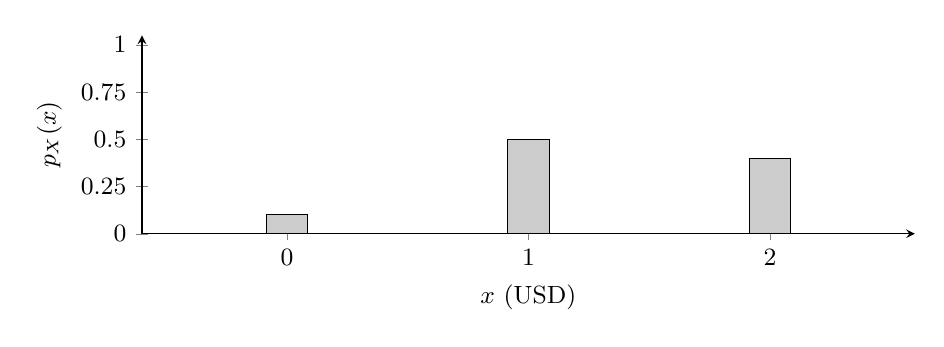
\begin{tikzpicture}\begin{axis}[width=.94\linewidth,height=4.1cm,axis lines=left,ymin=0,ymax=1.05,ytick={0,.25,.5,.75,1},xmin=-.6,xmax=2.6,xtick={0,1,2},xlabel={\GEHighlight{Quantity}{$x$ (USD)}},ylabel={\GEHighlight{Mass}{$p_X(x)$}},tick label style={font=\small},label style={font=\small}]\addplot[ybar,bar width=15pt,draw=cTwoMassColor,fill=cTwoMassColor!20] coordinates {(0,0.1) (1,0.5) (2,0.4)};\end{axis}\end{tikzpicture}\end{column}\end{columns}All masses are positive; $0.1+0.5+0.4=1$. Each mass keeps its numerical position and original spacing.
\end{frame}
\begin{frame}[t]{School shop: accumulate the PMF}
Write $F_X(x)=P(X\leq x)$ by accumulating in support order.
\[\begin{aligned}\visible<2->{F_X(0)&=\GEHighlight{Cumulative}{0.1},}\\\visible<3->{F_X(1)&=\GEHighlight{Cumulative}{0.1}+\GEHighlight{Mass}{0.5}=\GEHighlight{Cumulative}{0.6},}\\\visible<4->{F_X(2)&=\GEHighlight{Cumulative}{0.6}+\GEHighlight{Mass}{0.4}=\GEHighlight{Cumulative}{1}.}\end{aligned}\]
\visible<4->{Below the minimum no mass is included.}
\end{frame}
\begin{frame}[t]{School shop: CDF table and step graph}
\begin{columns}[T,onlytextwidth]\begin{column}{.36\textwidth}\begin{tabular}{cc}\toprule Cutoff interval & \GEHighlight{Cumulative}{$F_X(x)$} \\\midrule
$x<0$ & $\GEHighlight{Cumulative}{0}$ \\
$0\leq x<1$ & $\GEHighlight{Cumulative}{0.1}$ \\
$1\leq x<2$ & $\GEHighlight{Cumulative}{0.6}$ \\
$x\geq 2$ & $\GEHighlight{Cumulative}{1}$ \\
\bottomrule\end{tabular}\end{column}\begin{column}{.60\textwidth}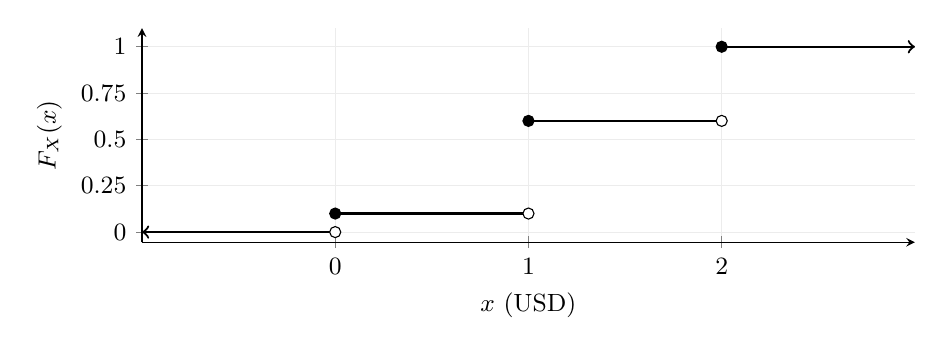
\begin{tikzpicture}\begin{axis}[cTwoCDF,width=.94\linewidth,height=4.3cm,xmin=-1,xmax=3,xtick={0,1,2},xlabel={\GEHighlight{Quantity}{$x$ (USD)}}]
\addplot[cTwoCDFColor,thick,<-] coordinates {(-1,0)(0,0)};
\addplot[cTwoCDFColor,thick] coordinates {(0,0.1)(1,0.1)};
\addplot[cTwoCDFColor,thick] coordinates {(1,0.6)(2,0.6)};
\addplot[cTwoCDFColor,thick,->] coordinates {(2,1)(3,1)};
\addplot[only marks,mark=*,cTwoCDFColor,mark size=2pt] coordinates {(0,0.1)(1,0.6)(2,1)};
\addplot[only marks,mark=*,cTwoCDFColor,mark options={fill=white},mark size=2pt] coordinates {(0,0)(1,0.1)(2,0.6)};
\end{axis}\end{tikzpicture}\end{column}\end{columns}
\end{frame}
\begin{frame}[t]{School shop: verify and interpret}
Check the defining properties before interpreting the heights.

\visible<2->{Nonnegative jumps make the CDF nondecreasing. Filled left/open right endpoints give right-continuity.}

\visible<3->{Tails at 0 and 1 give limits 0 and 1, with 1 attained at the maximum. Jumps $0.1,\ 0.5,\ 0.4$ match the PMF.}

\visible<4->{The mass at 1 groups both card methods; the CDF at 1 includes cash and both cards.}
\end{frame}
\begin{frame}[t]{School shop: connect mass and accumulation}
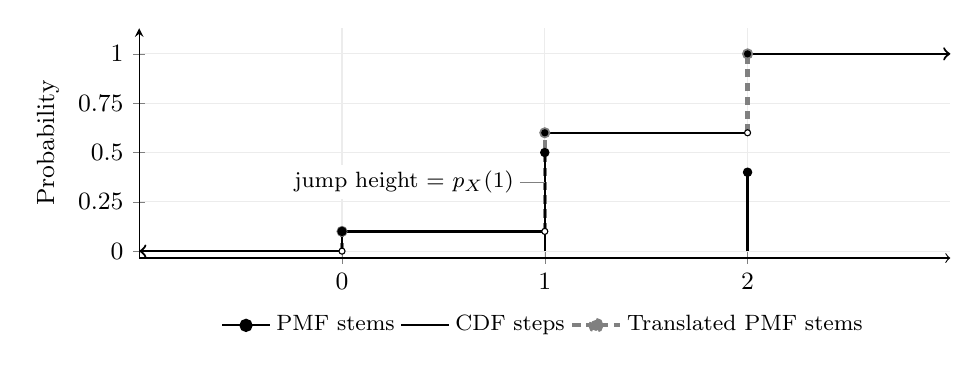
\begin{tikzpicture}
\begin{axis}[cTwoCombined,xmin=-1,xmax=3,xtick={0,1,2},xlabel={\GEHighlight{Quantity}{$x$ (USD)}}]
\cTwoPhantom{0}{.1}{0}
\cTwoPhantom{1}{.5}{1/10}
\cTwoPhantom{2}{.4}{3/5}
\cTwoMass{0}{.1}
\cTwoMass{1}{.5}
\cTwoMass{2}{.4}
\addplot[cTwoStep,<-] coordinates {(-1,0)(0,0)};
\addplot[cTwoStep] coordinates {(0,1/10)(1,1/10)};
\addplot[cTwoStep] coordinates {(1,3/5)(2,3/5)};
\addplot[cTwoStep,->] coordinates {(2,1)(3,1)};
\addplot[cTwoExcluded] coordinates {(0,0)(1,1/10)(2,3/5)};
\addplot[cTwoIncluded] coordinates {(0,1/10)(1,3/5)(2,1)};
\node[anchor=east,xshift=-9pt,font=\footnotesize,fill=white,inner sep=2pt] (jumpLabel) at (axis cs:1,7/20) {jump height = $p_X(1)$};
\draw[gray,thin] (jumpLabel.east) -- (axis cs:1,7/20);
\addlegendimage{cTwoMass,mark=*}\addlegendentry{PMF stems}
\addlegendimage{cTwoStep}\addlegendentry{CDF steps}
\addlegendimage{cTwoPhantom,mark=*}\addlegendentry{Translated PMF stems}
\end{axis}\end{tikzpicture}\par\medskip At $a=1$ USD, $0.6-0.1=0.5=p_X(1)$. Both card methods supply the mass at 1 USD. Read stems, translated guides and blue endpoints as before.
\end{frame}
\section{Summary}
\begin{frame}[t]{Keep the two representations connected}
A PMF separates distinct numerical results; equal fee values group mutually exclusive outcomes.

A CDF accumulates their masses from left to right. Its step heights include the cutoff.

Keep monetary values in USD and probabilities unitless. Retain numerical spacing and exact fractions or terminating decimals.
\[F_X(a)-F_X(a^-)=p_X(a).\]
\end{frame}
\section{Reminder}\begin{frame}[t]{General notation table legend}\small
\begin{tabularx}{\linewidth}{@{}l l X@{}}\toprule
Symbol or notation & Concept & Brief meaning\\\midrule
\GEHighlight{Quantity}{$X,x,a,S_X$} & \GEHighlight{Quantity}{Quantity} & Fee, value or cutoff, support; USD.\\
\GEHighlight{Mass}{$p_X(x)$} & \GEHighlight{Mass}{PMF} & One value; unitless; blue bars or stems.\\
\GEHighlight{Cumulative}{$F_X(x)$} & \GEHighlight{Cumulative}{CDF} & Through cutoff; unitless; related blue steps.\\
\GEHighlight{Cumulative}{$F_X(a^-)$} & Height before $a$ & Mass strictly below $a$; unitless.\\
$p_X(a)$ & Translated mass & From $F_X(a^-)$; pale dashed stem.\\
Filled / open dots & CDF endpoints & Filled: included; open: excluded.\\\bottomrule
\end{tabularx}\end{frame}\end{document}